\documentclass{mp}
\graphicspath{{07_rozklady/}}
\subtitle{Przykładowe rozkłady prawdopodobieństwa}
\begin{document}
\frame{\titlepage}

\begin{frame}{Rozkład dwupunktowy}
\only<1-2>
{
\begin{center}
\begin{tikzpicture}
\node[dice] (root) {?}
	child { node [diagram,below left=of root.center] {$X=-2$} edge from parent node[left] {$\leq 2$}}
	child { node [diagram,below right=of root.center] {$X=3$} edge from parent node[right] {$> 2$}};
\end{tikzpicture}
\end{center}
\[ P(X=-2)=\alert<1>{?} \qquad P(X=3)=\alert<1>{?} \]
}
\only<2->
{
\begin{block}{}
\begin{align*}
P(X=a)=p & \qquad P(X=b)=1-p \\
EX=\alert<2>{?} & \qquad DX=\alert<2>{?}
\end{align*}
\end{block}
\begin{block}<3->{Rozkład zero-jedynkowy}
\begin{align*}
P(X=1)=p & \qquad P(X=0)=1-p \\
EX=\alert<3>{?} & \qquad DX=\alert<3>{?}
\end{align*}
\end{block}
}
\end{frame}

\begin{frame}{Rozkład jednostajny dyskretny o parametrach $a$, $b$}
\begin{center}
\dice{1} \dice{2} \dice{3} \dice{4} \dice{5} \dice{6}
\end{center}
\begin{gather*}
P(X=k)=\alt<2->{\frac{1}{b-a+1}}{\alert{?}}\qquad k\in \{a,a+1,\ldots,b-1,b\} \\
\only<2->{EX=\frac{a+b}{2}\qquad DX=\sqrt{\frac{n^2-1}{12}}}
\end{gather*}
\end{frame}

\begin{frame}{Rozkład geometryczny}
\tabcolsep=0cm
\begin{tabular}{cccccccccc}
\includegraphics[width=.1\textwidth]{head.jpg} &
\includegraphics[width=.1\textwidth]{head.jpg} &
\includegraphics[width=.1\textwidth]{head.jpg} &
\includegraphics[width=.1\textwidth]{head.jpg} &
\includegraphics[width=.1\textwidth]{head.jpg} &
\includegraphics[width=.1\textwidth]{head.jpg} &
\includegraphics[width=.1\textwidth]{head.jpg} &
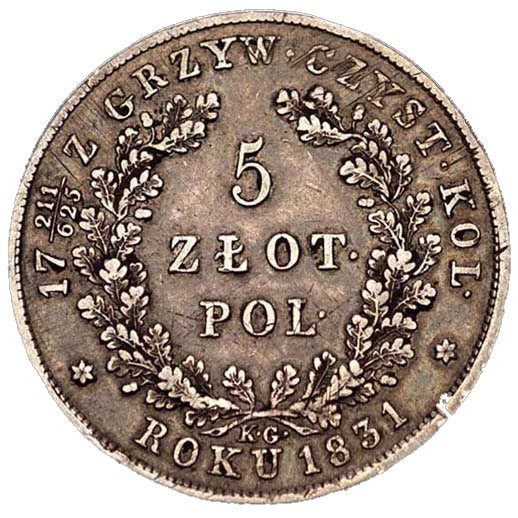
\includegraphics[width=.1\textwidth]{tail.jpg} &
\end{tabular}
\begin{gather*}
P(K=k)=(1-p)^{k-1}p \qquad k\in\{1,2,\ldots\} \\
EK=\frac{1}{p} \qquad DK=\frac{\sqrt{1-p}}{p}
\end{gather*}
\vfill
{\tiny Zdjecie monety z \url{http://commons.wikimedia.org/wiki/File:Powstanie_listopadowe_5_z\%C5\%82otych_1831.JPG} by \emph{Niki K} CC BY-SA 3.0}
\end{frame}

\begin{frame}{Oznaczanie pakietów sieciowych}
\begin{center}
\begin{tikzpicture}
\node (src) {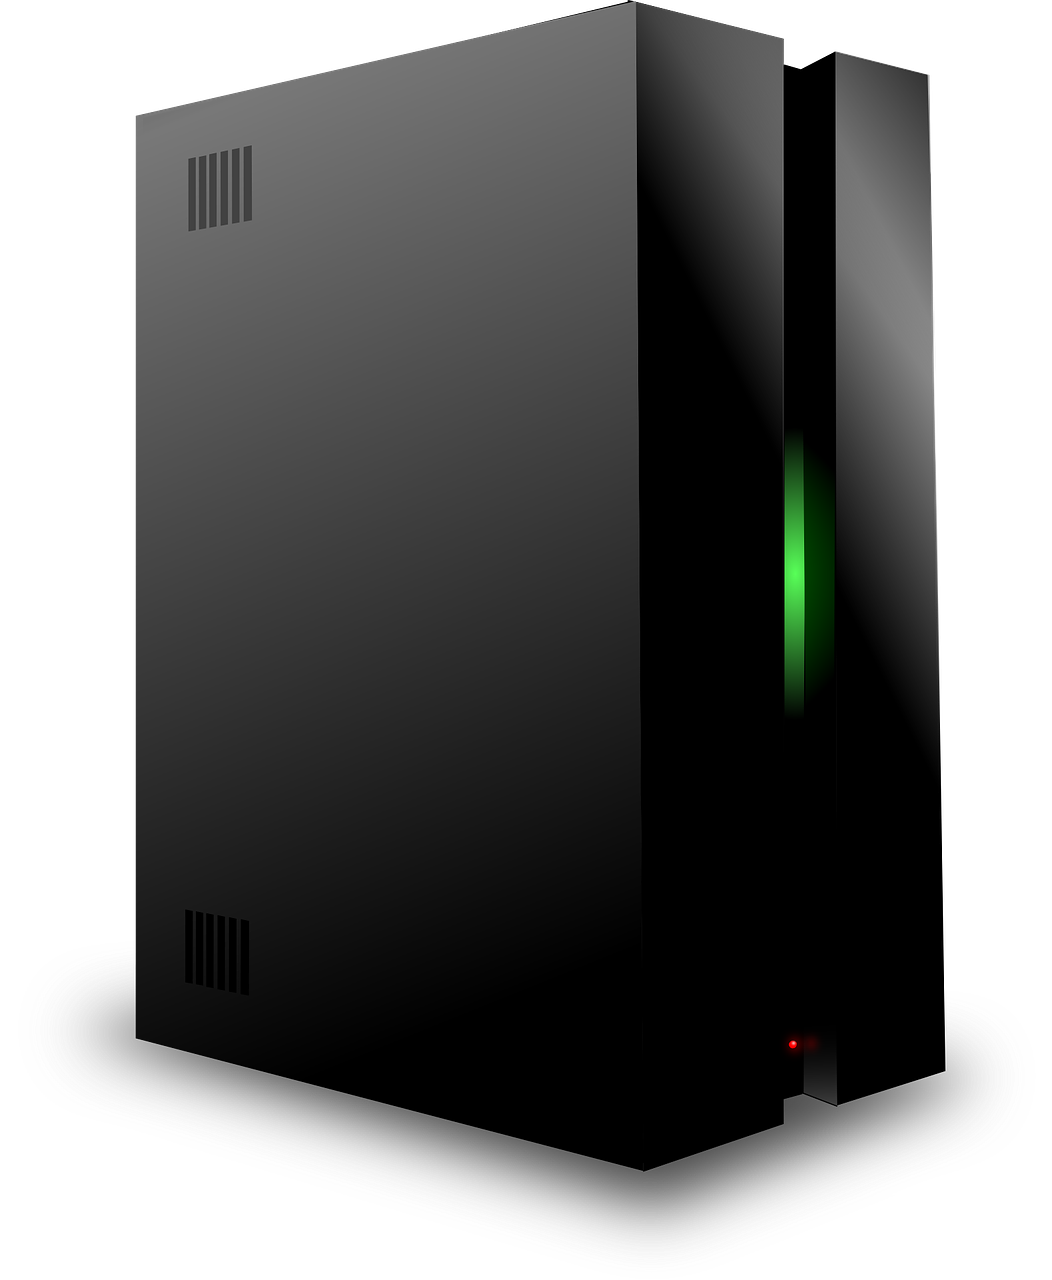
\includegraphics[width=.1\textwidth]{server.png}};
\node (a) [right=of src] {\includegraphics[width=.1\textwidth]{router.png}};
\node (b1) [above=of src] {\includegraphics[width=.1\textwidth]{router.png}};
\node (b2) [right=of b1] {\includegraphics[width=.1\textwidth]{router.png}};
\node (b3) [right=of b2] {\includegraphics[width=.1\textwidth]{router.png}};
\node (b4) [right=of b3] {\includegraphics[width=.1\textwidth]{router.png}};
\node (b5) [right=of b4] {\includegraphics[width=.1\textwidth]{router.png}};
\node (x) [right=of a] {};
\node (c) [right=of x] {\includegraphics[width=.1\textwidth]{router.png}};
\node (dst) [right=of c] {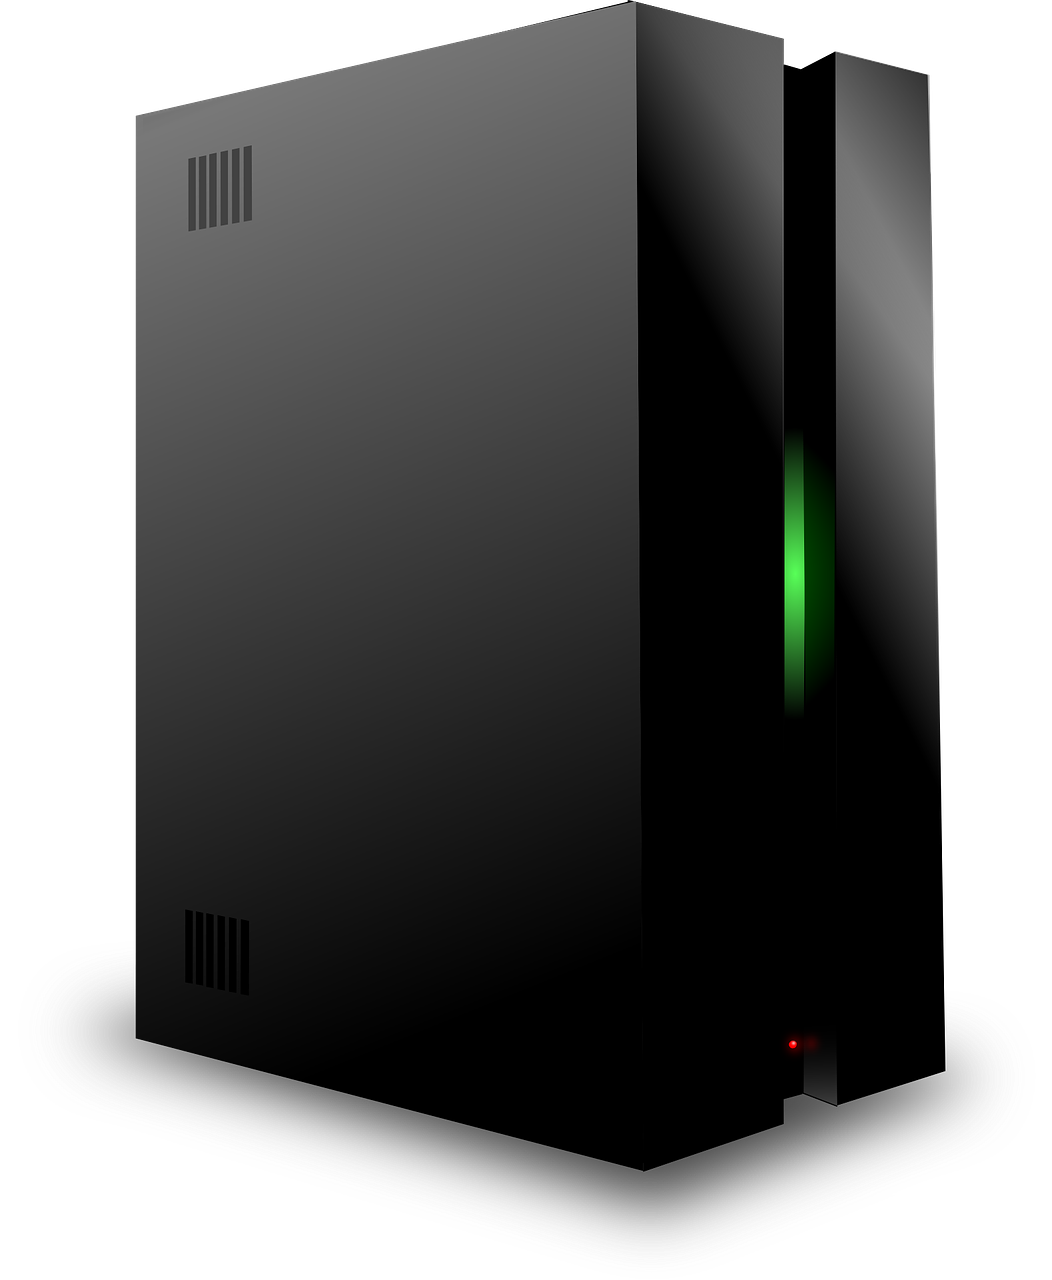
\includegraphics[width=.1\textwidth]{server.png}};
\draw (src.east)--(a.west) (c.east)--(dst.west) (a.east)--(c.west);
\draw (a.north west)--(b1.south east) (b1.east)--(b2.west) (b2.east)--(b3.west) (b3.east)--(b4.west) (b4.east)--(b5.west) (b5.south west)--(c.north east);
\end{tikzpicture}
\end{center}
\only<2>
{
\begin{center}
\begin{tabular}{|p{2cm}|p{2cm}|p{1cm}|p{2cm}|}
\hline
nadawca & odbiorca & licznik & \textcolor{color2}{router} \\
\hline
\multicolumn{4}{|c|}{dane} \\
\multicolumn{4}{|c|}{\ldots} \\
\hline
\end{tabular}
\end{center}
}
\only<2->{\[P(\textcolor{color2}{R}=k)=\frac{1}{n}\]}
\only<3->
{
	\begin{enumerate}
		\item<3-> Ile średnio trzeba odebrać pakietów, żeby poznać całą ścieżkę?
		\item<4-> Niech pakiet ma 64KB danych, a ścieżka 16 routerów. Ile średnio trzeba przesłać danych, żeby poznać całą ścieżkę?
		\item<4-> Ile pakietów wystarczy odebrać, żeby znać całą ścieżkę z prawdopodobieństwem przynajmniej $0{,}9$?
	\end{enumerate}
}
\vfill
\tiny{Rysunki z domeny publicznej, \url{http://pixbay.com}, użytkownik \emph{Nemo}}
\note<2>
{
$R$ id routera w nagłówku, $S_i$ prawdopodobieństwo, że $i$-ty router na ścieżce wpisze swój adres do nagłówka
\begin{gather*}
R=\arg\max_i S_i\\
P(S_i=1)=\frac{1}{i} \qquad P(S_i=0)=\frac{i-1}{i} \\
P(R=i)=P(S_i=1)\prod_{j\in\{i+1,\ldots,n\}} P(S_j=0)=\\
\frac{1}{i}\frac{\prod_{j\in\{i+1,\ldots,n\}}(j-1)}{\prod_{j\in\{i+1,\ldots,n\}}j}=\frac{1}{i}\frac{\frac{(n-1)!}{(i-1)!}}{\frac{n!}{i!}}=\frac{1}{n}
\end{gather*}
}
\note<3>
{
$X_i$ liczba pakietów, które trzeba odebrać, żeby poznać $i$-ty router, znając $i-1$ routerów
$X=\sum_{i=1}^n X_i$
$X_i$ ma rozkład geometryczny o prawdopodobieństwie sukcesu $\frac{n-(i-1)}{n}$ (znaczy, że trafimy na jeden z pozostałych $n-(i-1)$ nieznanych routerów)
\[P(X_i=k)=\left(\frac{i-1}{n}\right)^{k-1}\frac{n-(i-1)}{n} \]
zatem $EX_i=\frac{n}{n-(i-1)}$
\[EX=\sum_{i=1}^n EX_i=n\sum_{i=1}^n\frac{1}{n-(i-1)}=n\sum_{i=1}^{n}\frac{1}{i}=n(\ln n+\gamma) \qquad \gamma\in\left(0;1\right)\]
}
\note<4>
{
$P(X\leq k)\geq 0{,}9$
z nier. Markowa: $P(X>k\mu)<\frac{1}{k}$, zatem $P(X\leq k\mu)>1-\frac{1}{k}$, $1-\frac{1}{k}=0{,}9$, zatem $k=10$
Czyli wystarczy odebrać $10n(\ln n+1)$ pakietów. Jeżeli pakiet ma 64KB danych, a ścieżka 16 routerów, wychodzi, że potrzebujemy przesłać ok. 38MB

Nierówność Czebyszewa nie zastosuje się łatwo, bo wariancja jest dość upierdliwa w liczeniu:
Zmienne $X_i$ są niezależne, zatem $D^2X=\sum_{i=1}^n D^2X_i=\sum_{i=1}^n \frac{1-p_i}{p_i^2}=\ldots $
}
\end{frame}

\begin{frame}{Rozkład dwumianowy (Bernouliego)}
\tabcolsep=0cm
\begin{tabular}{cccccccccc}
\includegraphics[width=.1\textwidth]{head.jpg} &
\includegraphics[width=.1\textwidth]{head.jpg} &
\includegraphics[width=.1\textwidth]{head.jpg} &
\includegraphics[width=.1\textwidth]{head.jpg} &
\includegraphics[width=.1\textwidth]{head.jpg} &
\includegraphics[width=.1\textwidth]{head.jpg} &
\includegraphics[width=.1\textwidth]{head.jpg} &
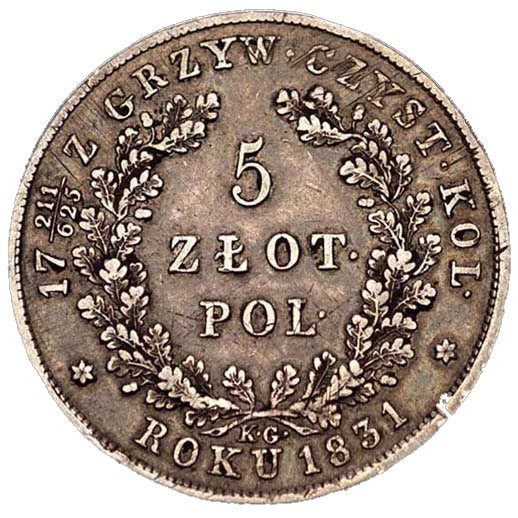
\includegraphics[width=.1\textwidth]{tail.jpg} &
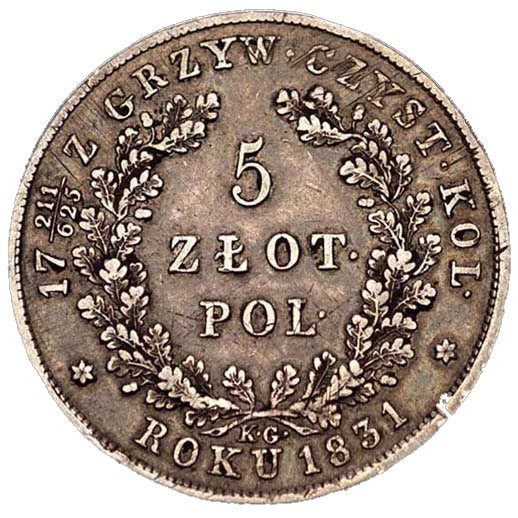
\includegraphics[width=.1\textwidth]{tail.jpg} &
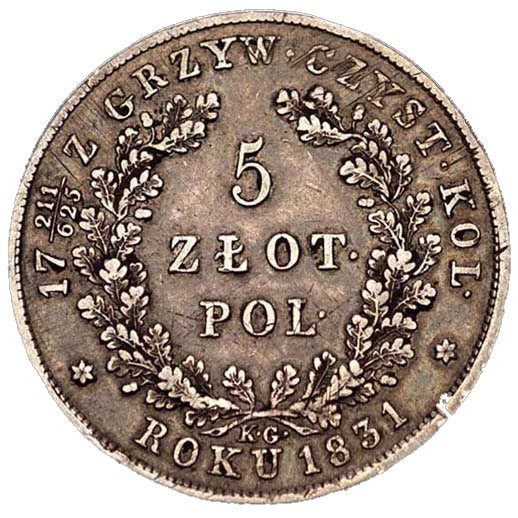
\includegraphics[width=.1\textwidth]{tail.jpg} \\
$X_1$ & $X_2$ & $X_3$ & $X_4$ & $X_5$ & $X_6$ & $X_7$ & $X_8$ & $X_9$ & $X_{10}$ \\
\end{tabular}
\begin{gather*}
P(X_i=1)=p \qquad P(X_i=0)=1-p \\
\only<2->{K=X_1+X_2+\ldots+X_n \\}
\only<3->{
	P(K=k)=\only<-5>{\alert<4->{?}}\only<6->{{n \choose k}}\only<5->{p^k(1-p)^{n-k}} \qquad k\in\{\only<3>{\alert{?}}\only<4->{0,1,\ldots,n}\}\\
}
\only<7->
{
	EK=\alert{?}\qquad DK=\alert{?}
}
\end{gather*}
\end{frame}
\begin{frame}{Rozkład Poissona}
\begin{tikzpicture}
\foreach \x in {0,...,49}
	\foreach \y in {0,...,4}
	\node at ($\x*(.02\textwidth,0)+\y*(0,.02\textwidth)$) {\ifnum \y<3 \includegraphics[width=.019\textwidth]{head.jpg}\else 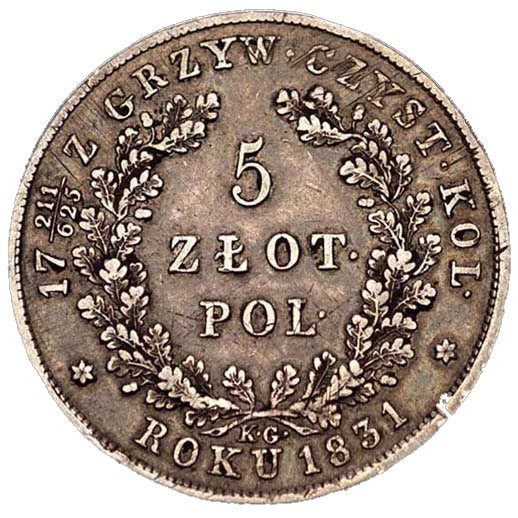
\includegraphics[width=.019\textwidth]{tail.jpg}\fi};
\end{tikzpicture}
\begin{gather*}
P(X=k)=e^{-\lambda}\frac{\lambda^k}{k!} \qquad k\in\{0,1,\ldots\}\quad \lambda\in\mathbb{R}_{+} \\
\only<2->{EX=\lambda\qquad DX=\sqrt{\lambda}}
\end{gather*}
\begin{block}<3->{Przybliżenie rozkładu Bernouliego rozkładem Poissona}
\[ \left( n\geq 50 \land p\leq 0{,}1 \land np\leq 10 \right) \to {n \choose k}p^k(1-p)^{n-k}\approx e^{-np}\frac{(np)^k}{k!} \]
\end{block}
\end{frame}
\begin{frame}{Tablice rozkładu Poissona}
\small
\tabcolsep=0.1cm
\input{poisson.tex}
\end{frame}
\end{document}
